%\title{emnlp 2017 instructions}
% File emnlp2017.tex
%
\PassOptionsToPackage{dvipdfmx}{graphicx} %or dvipdfm depending on the tex system

\documentclass[11pt,letterpaper]{article}
\usepackage{emnlp2017}
\usepackage{times}
\usepackage{latexsym}

\usepackage{graphicx}
\usepackage{amsmath}
\usepackage{amssymb}
%\usepackage[breaklinks=true,bookmarks=false]{hyperref}

% ==============CUSTOM PACKAGES (installed by Gota) ===================
% ref: https://github.com/jluttine/tikz-bayesnet
%\usepackage{tikz}
%\usetikzlibrary{bayesnet}
% ref: http://www.tapdancinggoats.com/latex-vector-notation.htm
\renewcommand{\vec}[1]{\mathbf{#1}}
%\usepackage{widetext}
\usepackage{array}
\usepackage{multirow}
\usepackage{longtable}
\usepackage{supertabular,booktabs}
\usepackage{tabularx}
\usepackage{tabulary}
\usepackage{xcolor}

\definecolor{_green}{rgb}{0.2745, 0.6235, 0.6157}
%\definecolor{_red}{rgb}{170,55,66}
\definecolor{_red}{rgb}{ 0.6667, 0.2157, 0.2588 }
\definecolor{test}{rgb}{ 0.6667, 0.2157, 0.2588 }
% ================================================================

% Uncomment this line for the final submission:
\emnlpfinalcopy

%  Enter the EMNLP Paper ID here:
\def\emnlppaperid{***}

% To expand the titlebox for more authors, uncomment
% below and set accordingly.
% \addtolength\titlebox{.5in}    

\newcommand\BibTeX{B{\sc ib}\TeX}


\title{Automatically Solving Word Algebra Problems with Structured Prediction Energy Networks}

% Author information can be set in various styles:
% For several authors from the same institution:
% \author{Author 1 \and ... \and Author n \\
%         Address line \\ ... \\ Address line}
% if the names do not fit well on one line use
%         Author 1 \\ {\bf Author 2} \\ ... \\ {\bf Author n} \\
% For authors from different institutions:
% \author{Author 1 \\ Address line \\  ... \\ Address line
%         \And  ... \And
%         Author n \\ Address line \\ ... \\ Address line}
% To start a seperate ``row'' of authors use \AND, as in
% \author{Author 1 \\ Address line \\  ... \\ Address line
%         \AND
%         Author 2 \\ Address line \\ ... \\ Address line \And
%         Author 3 \\ Address line \\ ... \\ Address line}
% If the title and author information does not fit in the area allocated,
% place \setlength\titlebox{<new height>} right after
% at the top, where <new height> can be something larger than 2.25in
\author{Arpit Jain\\ {\tt jain@umass.edu }  \And Gota Gando\\ {\tt ggando@umass.edu } \AND Krishna Prasad Sankaranarayanan\\ {\tt ksankaranara@umass.edu }  \And Nikhil Yadav\\
  {\tt nikhilyadav@umass.edu }}

\date{02/23/2018}

\begin{document}

\maketitle


% previous version
\if0
\section{Overview}
Solving word algebra problems automatically is a long-standing task in natural language processing (NLP). We plan to propose a new approach for solving algebra word problems automatically. In this task, the system needs to find a transformation from the given word problem into a set of equations which correctly represents the input word problem. To tackle this task, we apply structured prediction energy networks (SPENs), which is an energy based model where we can inject the structure knowledge of the task. We plan to start off from a simple feed-forward baseline model, and then evaluate and explore the possibilities of the SPEN model.
\fi

\begin{abstract}
To solve algebra word problems automatically, typical approaches find a transformation from the given word problem into a set of equations which correctly represents the input word problem. To approach this task, we apply structured prediction energy networks (SPENs), which is an energy based model where we can inject the structure knowledge of the task. We compare SPENs to a baseline of a simple feed-forward neural network model to determine the effectiveness of modeling structural dependencies in this problem.
\end{abstract}
%%%
%%%
\section{Introduction}
Algebra word problems in general describe some particular world situation and pose a question about it. In this project, we only consider the problems where we can use a system of equations to solve the questions. Figure \ref{algebra-example} shows one example of such problems. In this case, we can express the problem as a set of algebraic equations that descrbe the mathematical relationship of entities in the problem: for example $m = 4 \times n$ and $m-4 = 6 \times (n-4)$ where $m$ and $n$ represent the age of Maria and Kate, respectively. To answer the question, we need to solve these equations and get the solution. However, we focus on finding a mapping from the word problem into an equation system in this project, as there are many automated solvers for this process.
\begin{figure}[ht]
	\centering
	Maria is now four times as old as Kate.\\
Four years ago, Maria was six times as\\
old as Kate. Find their ages now.\\
	\caption{An example of word algebra problem.}
    \label{algebra-example}
\end{figure}
\subsection{Structured Prediction}
If we consider each character of the output equations as a random variable, then this task can be considered as a structured prediction task, as every output random variable would be dependent on some other variables. Furthermore, as both the input and output are sequences, we can also interpret this task as a sequence-to-sequnce task.

In many machine learning tasks, we try to predict $\textbf{y}$ given an input $\textbf{x}$. In some cases it is sufficient to use a discriminative function $F$ to predict the output such as $\textbf{y} = F( \textbf{x} )$. However, this model fails to model the structure of the output and the interactions among output components and may perform poor on more complex tasks. We can instead use \textit{an energy function} $E$ that both depends on $\textbf{x}$ and $\textbf{y}$ to model such structure and seek the optimal $\textbf{y}$ that minimizes the energy:
\begin{equation}
\hat{\mathbf{y}} = argmin_{\mathbf{y}} E( \mathbf{y}, \mathbf{x} )%E_{\mathbf{x}} (\mathbf{y})
\label{ebm0}
\end{equation}
Energy function can be seen as a scoring function that returns how compatible $\mathbf{x}$ and $\mathbf{y}$ are, or how likely they occur together.
One thing we need to note here is that there is no guarantee of the returning value of energy functions will be in the range of $\{ 0, 1\}$. One common way to address this problem and calibrate the energy is putting it through the Gibbs distribution.
\begin{equation}
P(Y|X) = \frac{ \exp{- \beta E(Y, X)} }{\int_{y \in \mathcal(Y)} \exp{- \beta E(y, X)}  }
\label{ebm1}
\end{equation}
However, it should be noted that this transformation is only possible when computing the integral term $\int_{y \in \mathcal(Y)} \exp{- \beta E(y, X)}$ is tractable.
%%%
%%%
\section{Related Works}
% TODO: COMPLETE THIS SECTION 
Solving word algebra problems automatically is a long-standing task in natural language processing (NLP).Solving word algebra problems automatically is a long-standing task in natural language processing (NLP). In this context, solving arithmetic word problems is of specific interest. One key challenge of solving algebra word problems is the lack of fully annotated data. Solving these problems require reasoning and logic across sentence boundaries to find a system of equations that precisely models the described semantic and mathematical relationships.

\citep{Kushman2014LearningTA} presented a baseline approach to solving algebra word problems using varied supervision, including either full equations or just the final answers . In this two step algorithm,  a template is first selected to match the overall structure of the equation system followed by which it is instantiated with numbers and nouns from the test. In this probabilistic inference mode, the probability of the answer is marginalized over the template selection and alignment.Following template induction wherein labeled equations are generalized to templates, inference is performed y beam search. Beam search provides a mapping to each template based on a canonical ordering. The results on primarily answer annotations ( weakly supervised data) were 70\%of the accuracies over the complete set of equations which clearly justified the benefits of supervision. 

\cite{roy2016solving} proposed a novel method for solving multi-step arithmetic word problems without the assistance of predefined annotations and templates. The algorithm is based on multiple classification problems on the target arithmetic equation and then combining these results to obtain the solutions. Grounding is the task ig taking an input word problem in the natural language and representing it as a formal language such as a set of equations, expression trees or states. This paper achieves grounding as a single step process. On the other hand,\citep{mitra2016learning}, splits this up into two parts. In the first step, the system learns to connect the assertions in a word problems to formula and in the second step, maps the formula into an algebraic equation.

\cite{KoncelKedziorski2015ParsingAW} formalizes solving algebraic word problems as that of generating and evaluating equation trees.Unlike in \cite{roy2017reasoning}, wherein a system for reasoning about quantities is introduced for arithmetic word problems involving only two values from the text and an arithmetic operator, this method (ALGES) learns to solve complex problems with multiple operands where the space of possible solutions is larger. Quantified sets (Qsets) are used a building block for equation trees to model natural language text quantities. These Qsets are combined with operator to yield a semantically augmented equation tree. With respect to grounding, the Qset properties are extracted and then ordered based on semantic and textual constraints followed by which Qsets are combined with arithmetic operators in an equation tree representation. The inference is to find the most likely equation tree with minimum violation of hard and soft constraints. This is facilitated by calculating a likelihood score for each operand t and the Qsets over which it is operated. Comparison results between template based methods and ALGES show
that although the template based methods are able to solve a wider range of problems than ALGES, ALGES fairs well fairs well even in systems with fewer repeated templates or less spurious lexical overlap between problems. In conclusion ALGES is a hybrid of template based and verb categorization methods.

\cite{UpChChYi16} demonstrates a state of the art approach for solving algebra word problems with little or no manual annotation of equations. In this novel structured-output learning ) algorithm (MixedSP), both explicit (eg., equations) and implicit(eg.,solutions) supervision signals are leveraged jointly.In the case of using algorithms that learn from implicit supervision, the system does not model directly the relation between input x and solution z. Also, multiple combinations of templates and alignments could end up with the same solution making implicit supervision slow, intractable and noisy. To overcome this limitation, MixedSP uses a standard structured prediction update procedure to find the best scoring candidate structures among the templates and alignments. Th algorithm starts with just explicit signals since it leads to a better intermediate model which later allows exploring the output space more efficiently using the implicit signals. The results clearly demonstrate that a joint learning approach benefits from noisy implicit supervision. The accuracies are represented for Explicit, Implicit, Pseudo, Pseudo + Explicit and MixedSP. Mixed SP outperforms it's counterparts even without manual annotation.



%%%
%%%
\section{Problem Definition}
\subsection{Template}
Following \cite{Kushman2014LearningTA}, we define the space of possible equations by a set of "templates". A template represents a structure for a set of equations for an algebra problem, consisting of slots for unknown variables and coefficients. As we express equations as a sequence of symbol indices, there can be many possible correct equations. Therefore, we assume that each text problem has only one correct set of equations, and express the structure with a template. Figure \ref{template} shows an example of template selection and instantiation. In this case the template has $u_i$ slots that represent unknown variables, and $n_j$ slots for coefficients values. In this scheme, transformation of word problems to equations as a two step process. First, a template is selected to define the structure of the target equation system. Second, the selected template is instantiated with actual texts for unknowns and values for coefficients. 
\begin{figure*}[ht]
	\centering
	%\includegraphics[bb=0 0 912 419, natheight=5cm]{figs/fig_encdec.pdf}%scale=0.8, 
	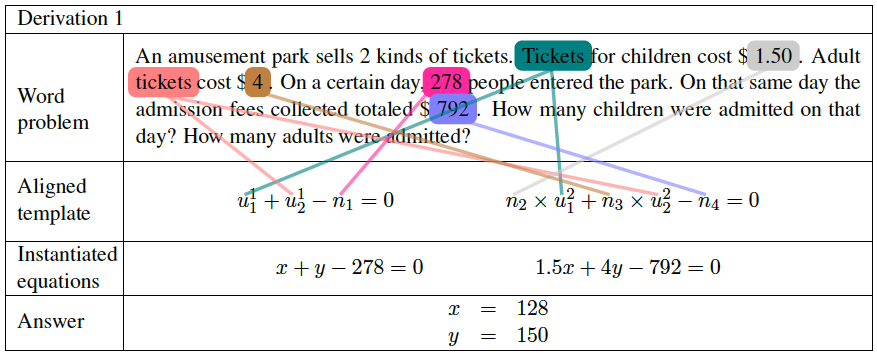
\includegraphics[bb=0 0 877 353, scale=0.5]{template.png}%scale=0.8, 
    \caption{The structure of the baseline model. Cited from \cite{Kushman2014LearningTA}}
    \label{template}
\end{figure*}
\subsection{Derivation}
In this section, we review the formulation described in \cite{Kushman2014LearningTA} and \cite{UpChChYi16}. We denote the input word problem as $\textbf{x}$, and the output as $\textbf{y}$. We call the output as a derivation, which consists of a template $T$ and an alignment $A$. Therefore we can express the output as $\textbf{y} = (T, A)$. More specifically, template $T$ is a set of equations $= \{t_0, ..., t_l\}$, and an alignment $A$ is defined as a set of pairs $(w, s)$, where where $w$ is a token in $\textbf{x}$ and $s$ is a slot instance in $T$.
%%%
%%%
\section{Methods}
\subsection{Scoring function}
We first describe our manually constructed scoring function, which is used for both the baseline model and SPEN. This function takes in as a predicted derivation and the true derivation, and returns the score of how good the prediction is. We also pass the problem text and the solution (e.g. $x=2, y=3$) of the true equation to this function so that it can utilize the full information. It first compares the predicted template index with the true template index, and punishes significantly if the predicted index differs from the true index. This is because if the derivation uses a different template, two derivations would be completely different. If the template index matches, then the function examines how the coefficients are matching; for each coefficient slot, it computes the distance between the predicted token index and the true token index, and add a negative value to the score proportional to the distance. Finally, the function solves the predicted equations and checks if the solutions are matching the actual solutions of the true equations. If the solution does not match, it penalizes the final score. Often times, the alignments in the predicted derivation do not point to actual number words such as "two" or "1,000". In those cases we search for the nearest number word in the problem text, and build the predicted equation with the filled out coefficients.
% TODO: Add more details here
\subsection{Baseline model}
% [NOTE] The mlp model is more of a preliminary experiment so here we need to talk about the greedy baseline, which we actually compare the result of SPEN with.
To evaluate the performance of SPEN, We build a greedy baseline which determines the prediction for a word problem component by component. It first determines the component for template index by checking the scores from all the possible indices with the above mentioned scoring function. After fixing the template, it then proceeds with determining the value for each coefficient slot greedily.
%We plan to use two baseline models. One is a regular feed-forward neural network that predicts the output equations directly from the input, interpreting the task as a black-box sequence-to-sequence task. Another baseline is also a neural network that jointly predicts derivation of templates and its alignments. In both cases, first the input text problem is put through a word embedding layer and a vector is assigned to each word. The first baseline then predicts the output directly after forwarding through several intermediate layers. The second baseline model on the other hand, tries to predict the template structure and its alignments at the same time. This is performed by constructing a derivation vector where the first element denotes the index of the predicted template and the other elements denote the textual or integer values of each unknowns / coefficients in the selected template.
\subsection{SPEN}
%Unlike feed-forward approaches, 
%As with other EBMs, SPEN tries to predict $y$
Structured Prediction Energy Networks (SPENs) \cite{DBLP:journals/corr/BelangerM15}\cite{belanger2017end} are one of the energy-based models (EBMs) that performs structured prediction, such as conditional random fields (CRFs), structured perceptrons, and structured SVMs (SSVMs).
There are two main differences betwen SPEN and other energy-based models. First, SPENs can learn non-linear energy functions, as it is parameterized by a deep neural network. Similar to other EBMs, SPEN also tries to predict $y$ that minimizes the energy function. While EBMs listed above usually assume a restricted graphical structure such as a chain or a tree and consider a linear energy function, SPEN instead considers a general energy function and assumes the non-convexity. Then, it approximates the optimal $\mathbf{y}$ with gradient descent:
\begin{equation}
\mathbf{\bar{y}} = argmin_{\mathbf{\bar{y}}} E( \mathbf{\bar{y}}, \mathbf{x} )
%Ex(y) subject to y \in \{0, 1\}
\end{equation}
\begin{equation}
\mathbf{y}^{t+1} = \mathbf{y}^t - \eta \frac{ \partial E }{ \partial \mathbf{y^t}}
\end{equation}
Additionally, SPENs are much more efficient at the inferene stage where the model predicts a candidate output $\bar{\mathbf{y}}$, as SPENs use gradient descent to approximate an optimal $\bar{\mathbf{y}}$ instead of using computationally expensive searching methods such as viterbi algorithm or beam search.
%%
\subsection{Architecture of SPEN}
Although SPEN can take general energy functions, in this work we consider the energy function consists of the global energy and the sum of local energies as follows:
\begin{align}
E_x^{local}(\bar{y}) = \sum^L_{i=1} \bar{y_i} b_i^T F(x) \\
E_x^{global}(\bar{y}) = c_2^T g(C_1 \bar{y})
\end{align}
where $g$ is a non-linearity function, each $b_i$ is a vector of parameters for each label, and the product $C_1 \bar{y}$ is a set of learned affine (linear + bias)
measurements of the output.

We give the same representation of $y$ as described in the baseline section to this energy network.
% TODO: ADD MORE DETAILED EXPLANATION WITH EQUATIONS
%%
%%
\subsection{Rank-based loss}
The traditional SPEN framework uses the SSVM loss:
\begin{equation}
\sum_{ \{x_i,y_i\} } \max_y \big[ \Delta(y_i, y) - E_{x_i}(y) + E_{x_i}(y_i) \big]_+
\end{equation}
Here, $+[ \cdot ]$ denotes the max function. However, this loss requires the full annotation for derivations. As our dataset only contains partial annotations for alignments, we use a rank-based loss which is defined as below:
{ \small
\begin{equation}
\min_\mathbf{w} \sum_{ \mathbf{x} \in \mathcal{D} } \big[ \alpha(V(\mathbf{y}_h, \mathbf{x}) - V(\mathbf{y}_l, \mathbf{x})) - E_{\mathbf{w}}(\mathbf{y}_h, \mathbf{x}) + E_{\mathbf{w}}(\mathbf{y}_l, \mathbf{x})  \big]_+
\end{equation}
}
Where $V$ is the value from the scoring function. The intuition of this loss is that we would like to approximate the scoring function with the energy networks. One big advantage of this approach is that, unlike the raw scoring function energy networks are differentiable and have less local optima. Therefore, we do not need to enumerate all the possible configurations for $y$ and we can obtain the minimum $y$ that minimizes the energy function automatically, as described in Section 4.3.
%
\begin{figure}[ht]
	\centering
	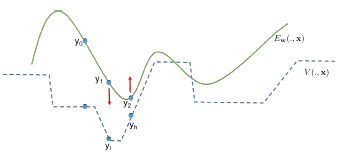
\includegraphics[bb=0 0 338 154, scale=0.5]{rank-based_loss}
    \caption{The illustration of the rank-based loss.}
    \label{spen-architecture}
\end{figure}
%%%
%%%
\section{Experiments}
\subsection{Datasets}
We plan to use two datasets; the ALG-514 dataset proposed by \cite{Kushman2014LearningTA} which contains 514 word problems, and the DRAW dataset provided by Microsoft that contains about 1000 independent examples. One issue we are currently aware of these datasets is that ,while they include template structure of output equations for each problem, they do not provide the mapping of unknowns to text values. We plan to manually annotate such alignment information on these datasets so that we can fully make use of the template structure and its alignments.
\subsection{Preliminary experiment}
To check if our structure of the output $\mathbf{y}$ is actually learnable by a neural network, we first trained a small MLP model with a subset of the ALG-514 dataset. The network consists of one embedding layer, one dense layer and 7 softmax layers. We trained the network with a joint loss which is the sum of all the losses from each softmax layer. The embedding layer is initialized with the 50 dimensional Glove vector. We confirmed that the network successfully overfit to the first 10 examples of the dataset and achieved 1.0 accuracy and 0.0 loss value for the train set after 50 epochs.
%
\subsection{Experimental settings for SPEN}
Next, we evaluated the performance of the baseline model and the SPEN with the full dataset of ALG-514. We show the architecture of the energy networks in Figure \ref{spen-architecture}. We implemented our scoring function using sympy, and we trained the SPEN with both the SSVM loss and the rank-based loss. On training SPEN, we first trained a neural network with a supervised sequence-to-sequnce task with the dataset and fine-tuned the glove initialized embedding layer. Then, we initialized the embedding layer of SPEN with the pretrained deep neural network and trained the model with a rank-based loss. Hyperparameters used during the training are shown in Table \ref{params}.
\begin{figure}[ht]
	\centering
	%\includegraphics[bb=0 0 912 419, natheight=5cm]{figs/fig_encdec.pdf}%scale=0.8, 
	\hspace*{-10mm}
	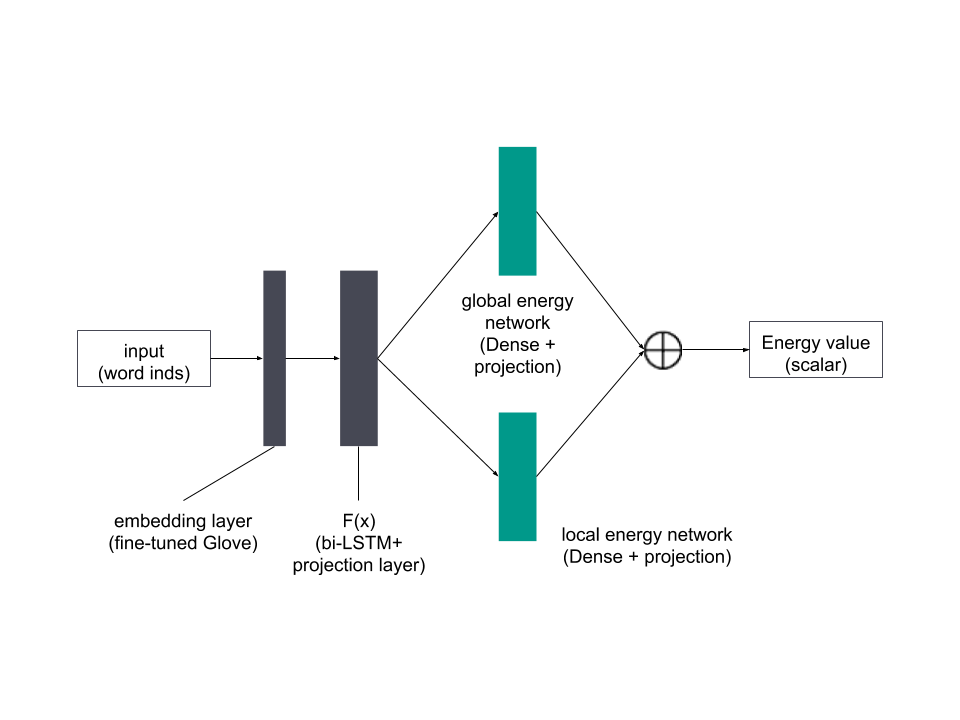
\includegraphics[bb=0 0 960 720, scale=0.28]{spen_architecture.png}%scale=0.8, 
    \caption{The architecture of the SPEN model used in the experiment.}
    \label{spen-architecture}
\end{figure}
%
\begin{table}[]
\centering
\caption{Hyperparameters of the model}
\label{params}
\begin{tabular}{ll}
\textbf{Parameter name} & \textbf{Value} \\
Learning rate           & 0.001          \\
Embedding dim           & 50             \\
Batch size              & 100            \\
Inference iterations    & 50             \\
Inference rate          & 0.1            \\
Margin weight           & 100           
\end{tabular}
\end{table}
% TODO: write more details
%%%
%%%
\section{Results and Discusstion}
Table \ref{result} shows the accuracies for the second experiment. Both approaches of the SPEN outperformed the greedy baseline model, and the model trained with the rank-based loss achieved about a 4\% higher accuracy. However, this result is very lower than the accuracy reported by \cite{Kushman2014LearningTA},
\begin{table*}[]
\centering
\caption{Experimental results with the ALG-514 dataset. Each cell represents the accuracy of a method.}
\label{result}
\begin{tabular}{lll}
\textbf{Baseline (greedy)} & \textbf{SPEN (SSVM loss)} & \textbf{SPEN (Rank-based loss)} \\
0.0127                     & 0.0898                    & 0.1323                         
\end{tabular}
\end{table*}
% TODO: Write our analysis on the results or problems of the current scoring function, etc.
%%%
%%%
\section{Planned works}
As the greedy baseline performed very pooly, we plan to implement a better baseline using beam search, to see if the SPEN's performance is actually higher than much simpler methods. We are also suspecting that our scoring function is not sophisticated enough, as we achieved lower accuracies than we expected, and plan to improve our scoring function. Lastly, we are planning to explore better architectures for energy networks and tune the optimization and inference parameters of SPEN to obtain a higher accuracy.
% Write our plan of improving the scoring function??
%%%
%%%
% previous sections in the proposal
\if0
\section{Evaluation}
Following the existing works, we evaluate the model's performance with the overall accuracy on the ALG-514 and DRAW datasets. The predicted equation system is marked as correct if all the characters of the output exactly matches the ground truth equations. We also plan to evaluate the accuracy on several subsets of word problems to further analyze problems the model can perform well.
%%%
%%%
\section{Datasets}
We plan to use two datasets; the ALG-514 dataset proposed by \cite{Kushman2014LearningTA} which contains 514 word problems, and the DRAW dataset provided by Microsoft that contains about 1000 independent examples. One issue we are currently aware of these datasets is that ,while they include template structure of output equations for each problem, they do not provide the mapping of unknowns to text values. We plan to manually annotate such alignment information on these datasets so that we can fully make use of the template structure and its alignments.
%%%
%%%
\section{Scope}
Although it might be interesting to explore how we can improve the model itself, we limit the scope of this project to applying and evaluating the baseline MLP and SPEN model. Application of the SPEN includes designing structured representation of the output variable $y$. We are also planning to utilize the "implicit" data samples described in \cite{UpChChYi16}, which only contain the solutions of equations and not equation themselves if we have time after evaluating the baselines and the SPEN model. In this approach, we hope to jointly learn from data samples with equation labels and without such labels.
\fi
%
\nocite{*}
\bibliography{696ds_bib}
\bibliographystyle{emnlp_natbib}

\end{document}
